\section{Lancement de la partie}
Deux cas distincts peuvent se présenter lors du lancement de la partie :
\begin{itemize}
  \item La création de partie
  \item Le chargement de partie
\end{itemize}
Ces deux cas seront implémentés via le design pattern monteur, comme convenu avec ce qui nous était imposé.
On peut en effet trouver des étapes similaires lors de chacun d'entre-eux., telle qu'une étape de création de carte, la création de 2 joueurs, de leurs unités, etc.
Nous étudierons donc ces deux cas l'un après l'autre.

\subsection{Création de partie}
La création de partie utilise les informations passées par le menu principal pour créer une nouvelle partie.
Ces informations regrouppent le nom des joueurs, leur peuple et la taille de la carte.
La méthode de création est appelée par le monteur de partie, et celle-ci est détaillé sur le diagramme de séquence \ref{fig:newGame}.
\begin{figure}[h!]
    \centering
    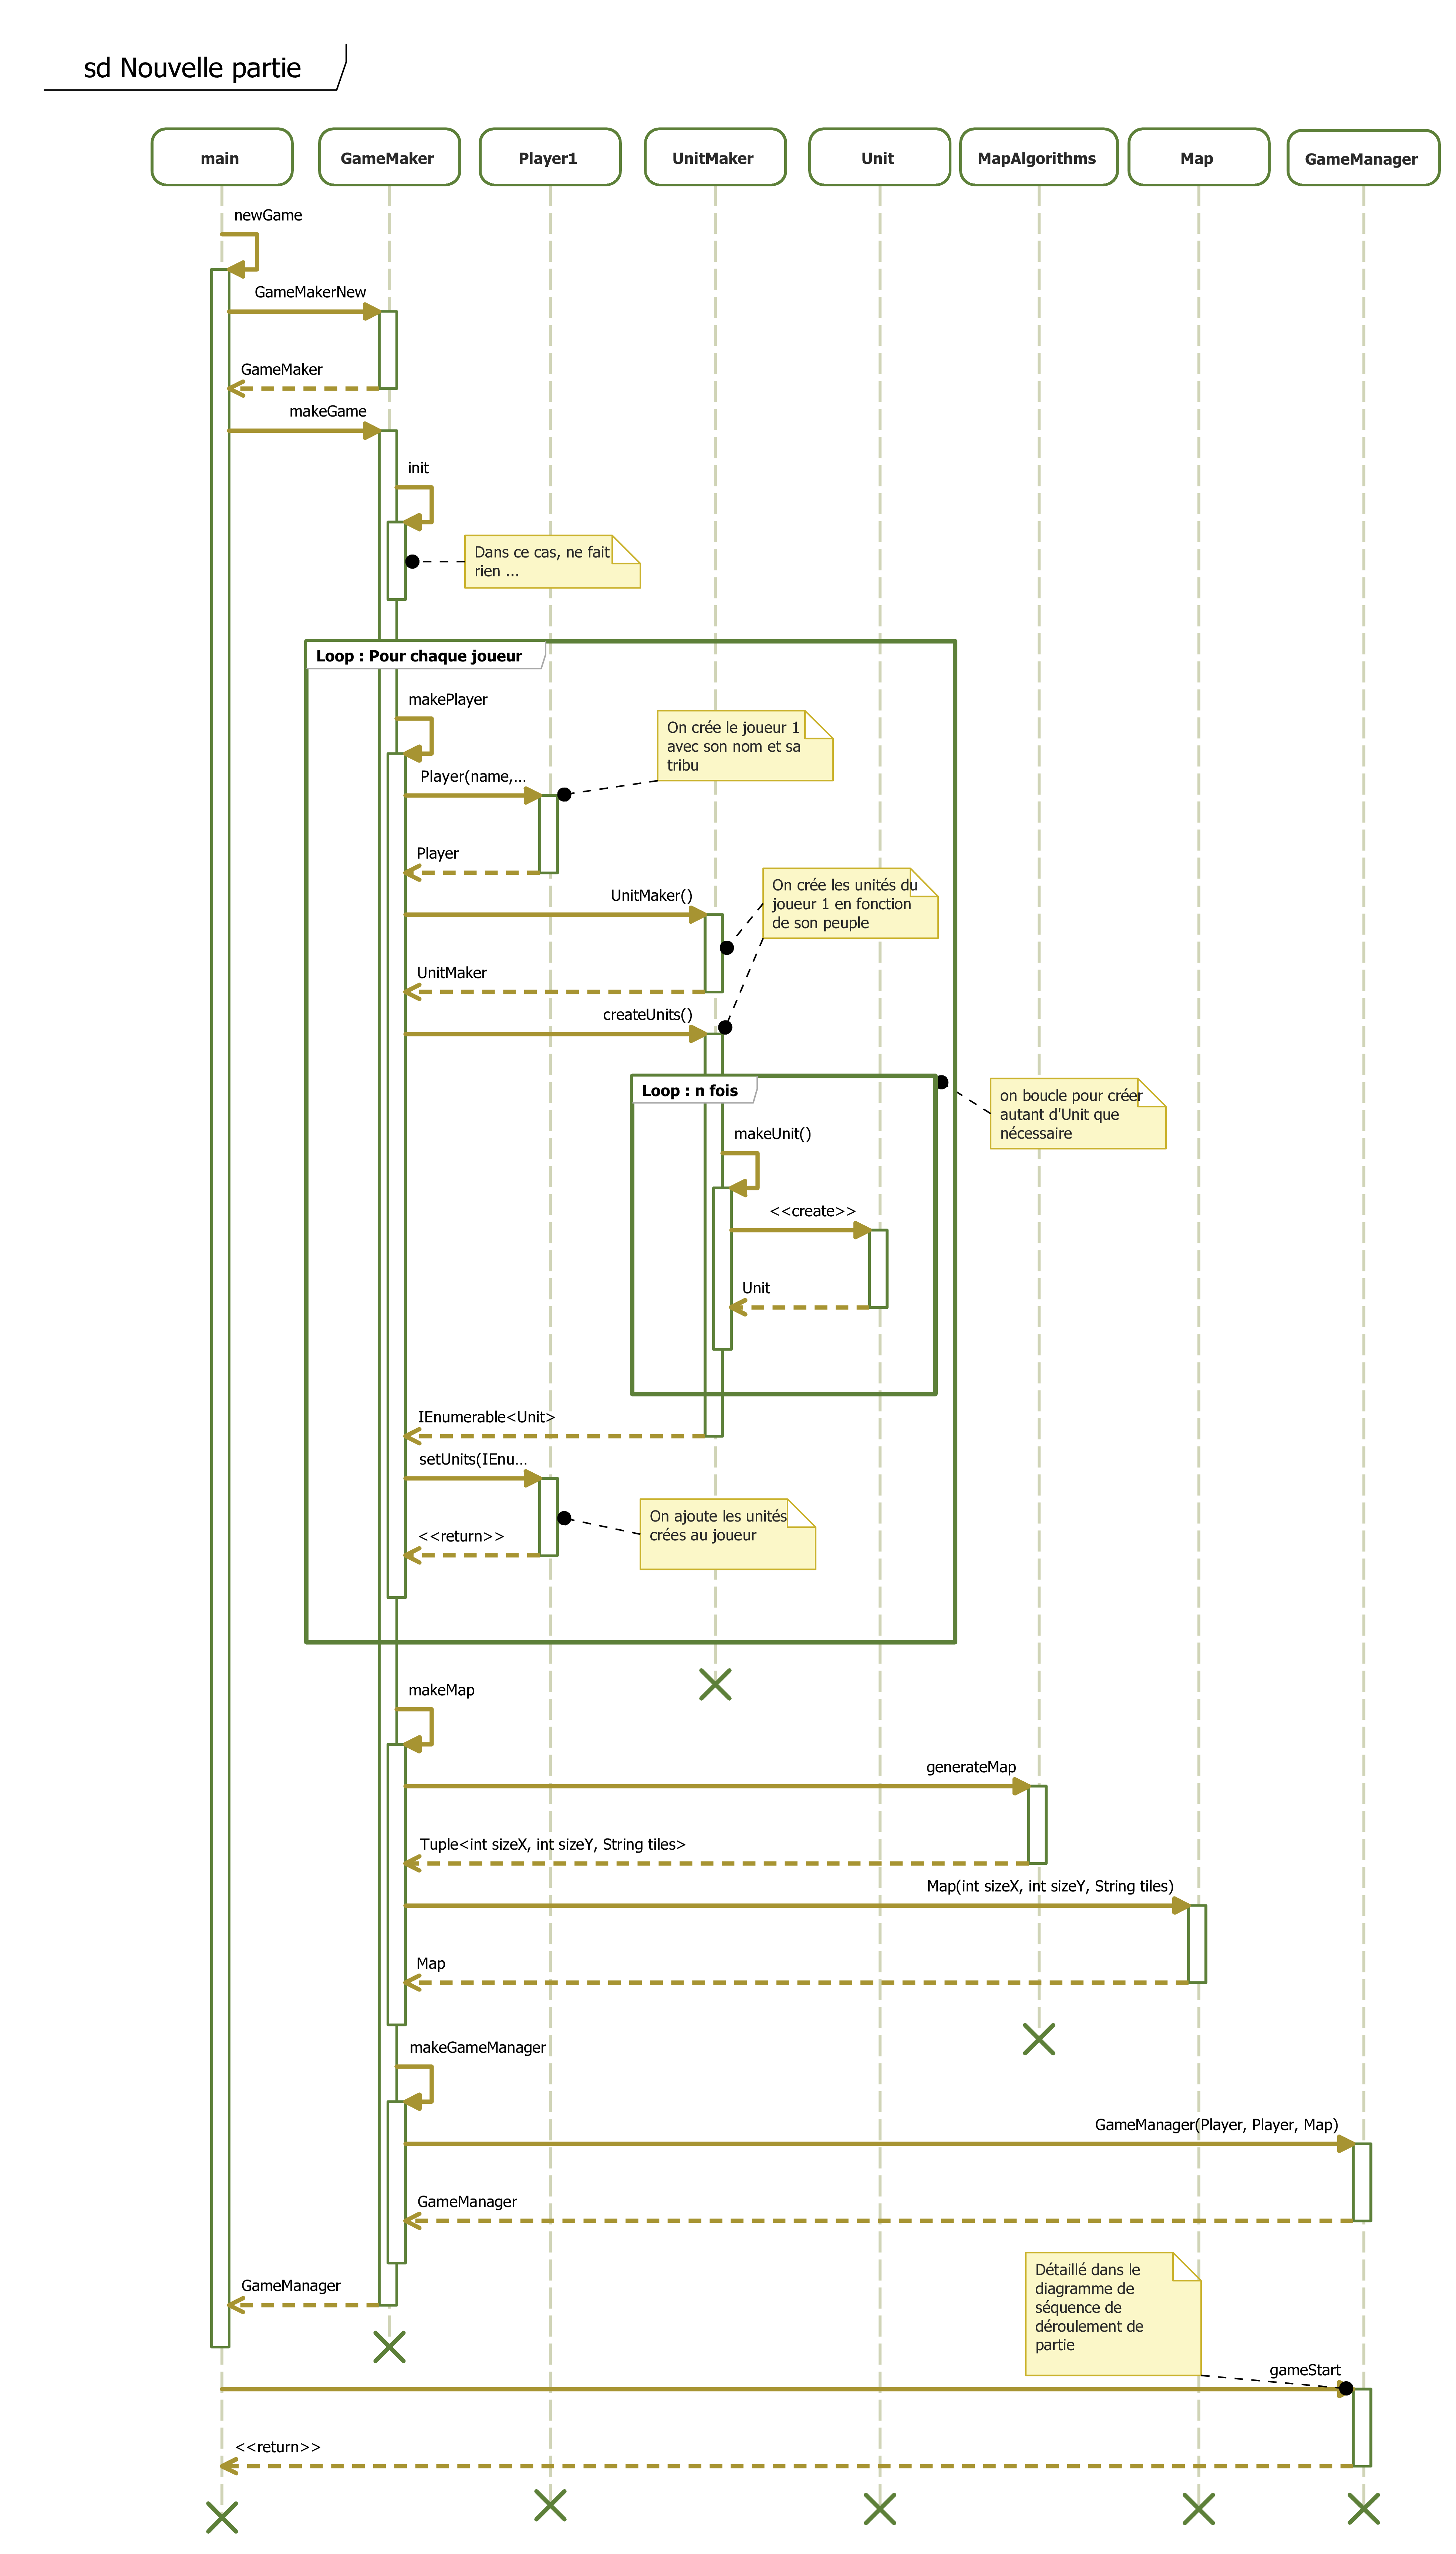
\includegraphics[width=0.8\textwidth]{res/NouvellePartie.png}
    \caption{Creation de partie}
    \label{fig:newGame}
\end{figure}

\subsection{Chargement de partie}
Le chargement de sauvegarde permet à un joueur de reprendre une partie en cours. La restauration de partie s'effectue en trois étapes :
\begin{itemize}
  \item Restauration des joueurs : Les noms de joueurs, leur tribu, leurs points.
  \item Restauration des unités : Leurs points de vie, propriétaire et leur position.
  \item Restauration de l'état du jeu : Tour de jeu global et joueur courant.
\end{itemize}
La récupération de l'état du jeu permet ainsi de reprendre une partie à l'endroit exact où on l'avait laissé.
Il est ainsi possible de charger une partie sauvée entre deux mouvements d'unités.
Le monteur de partie réalisant le chargement doit faire appel à un système de chargement de sauvegarde; celui-ci sera détaillé davantage au cours de ce rapport. 
Les méthodes appelées par le monteur sont détaillées sur le diagramme de séquence \ref{fig:loadGame}.
\begin{figure}[h!]
    \centering
    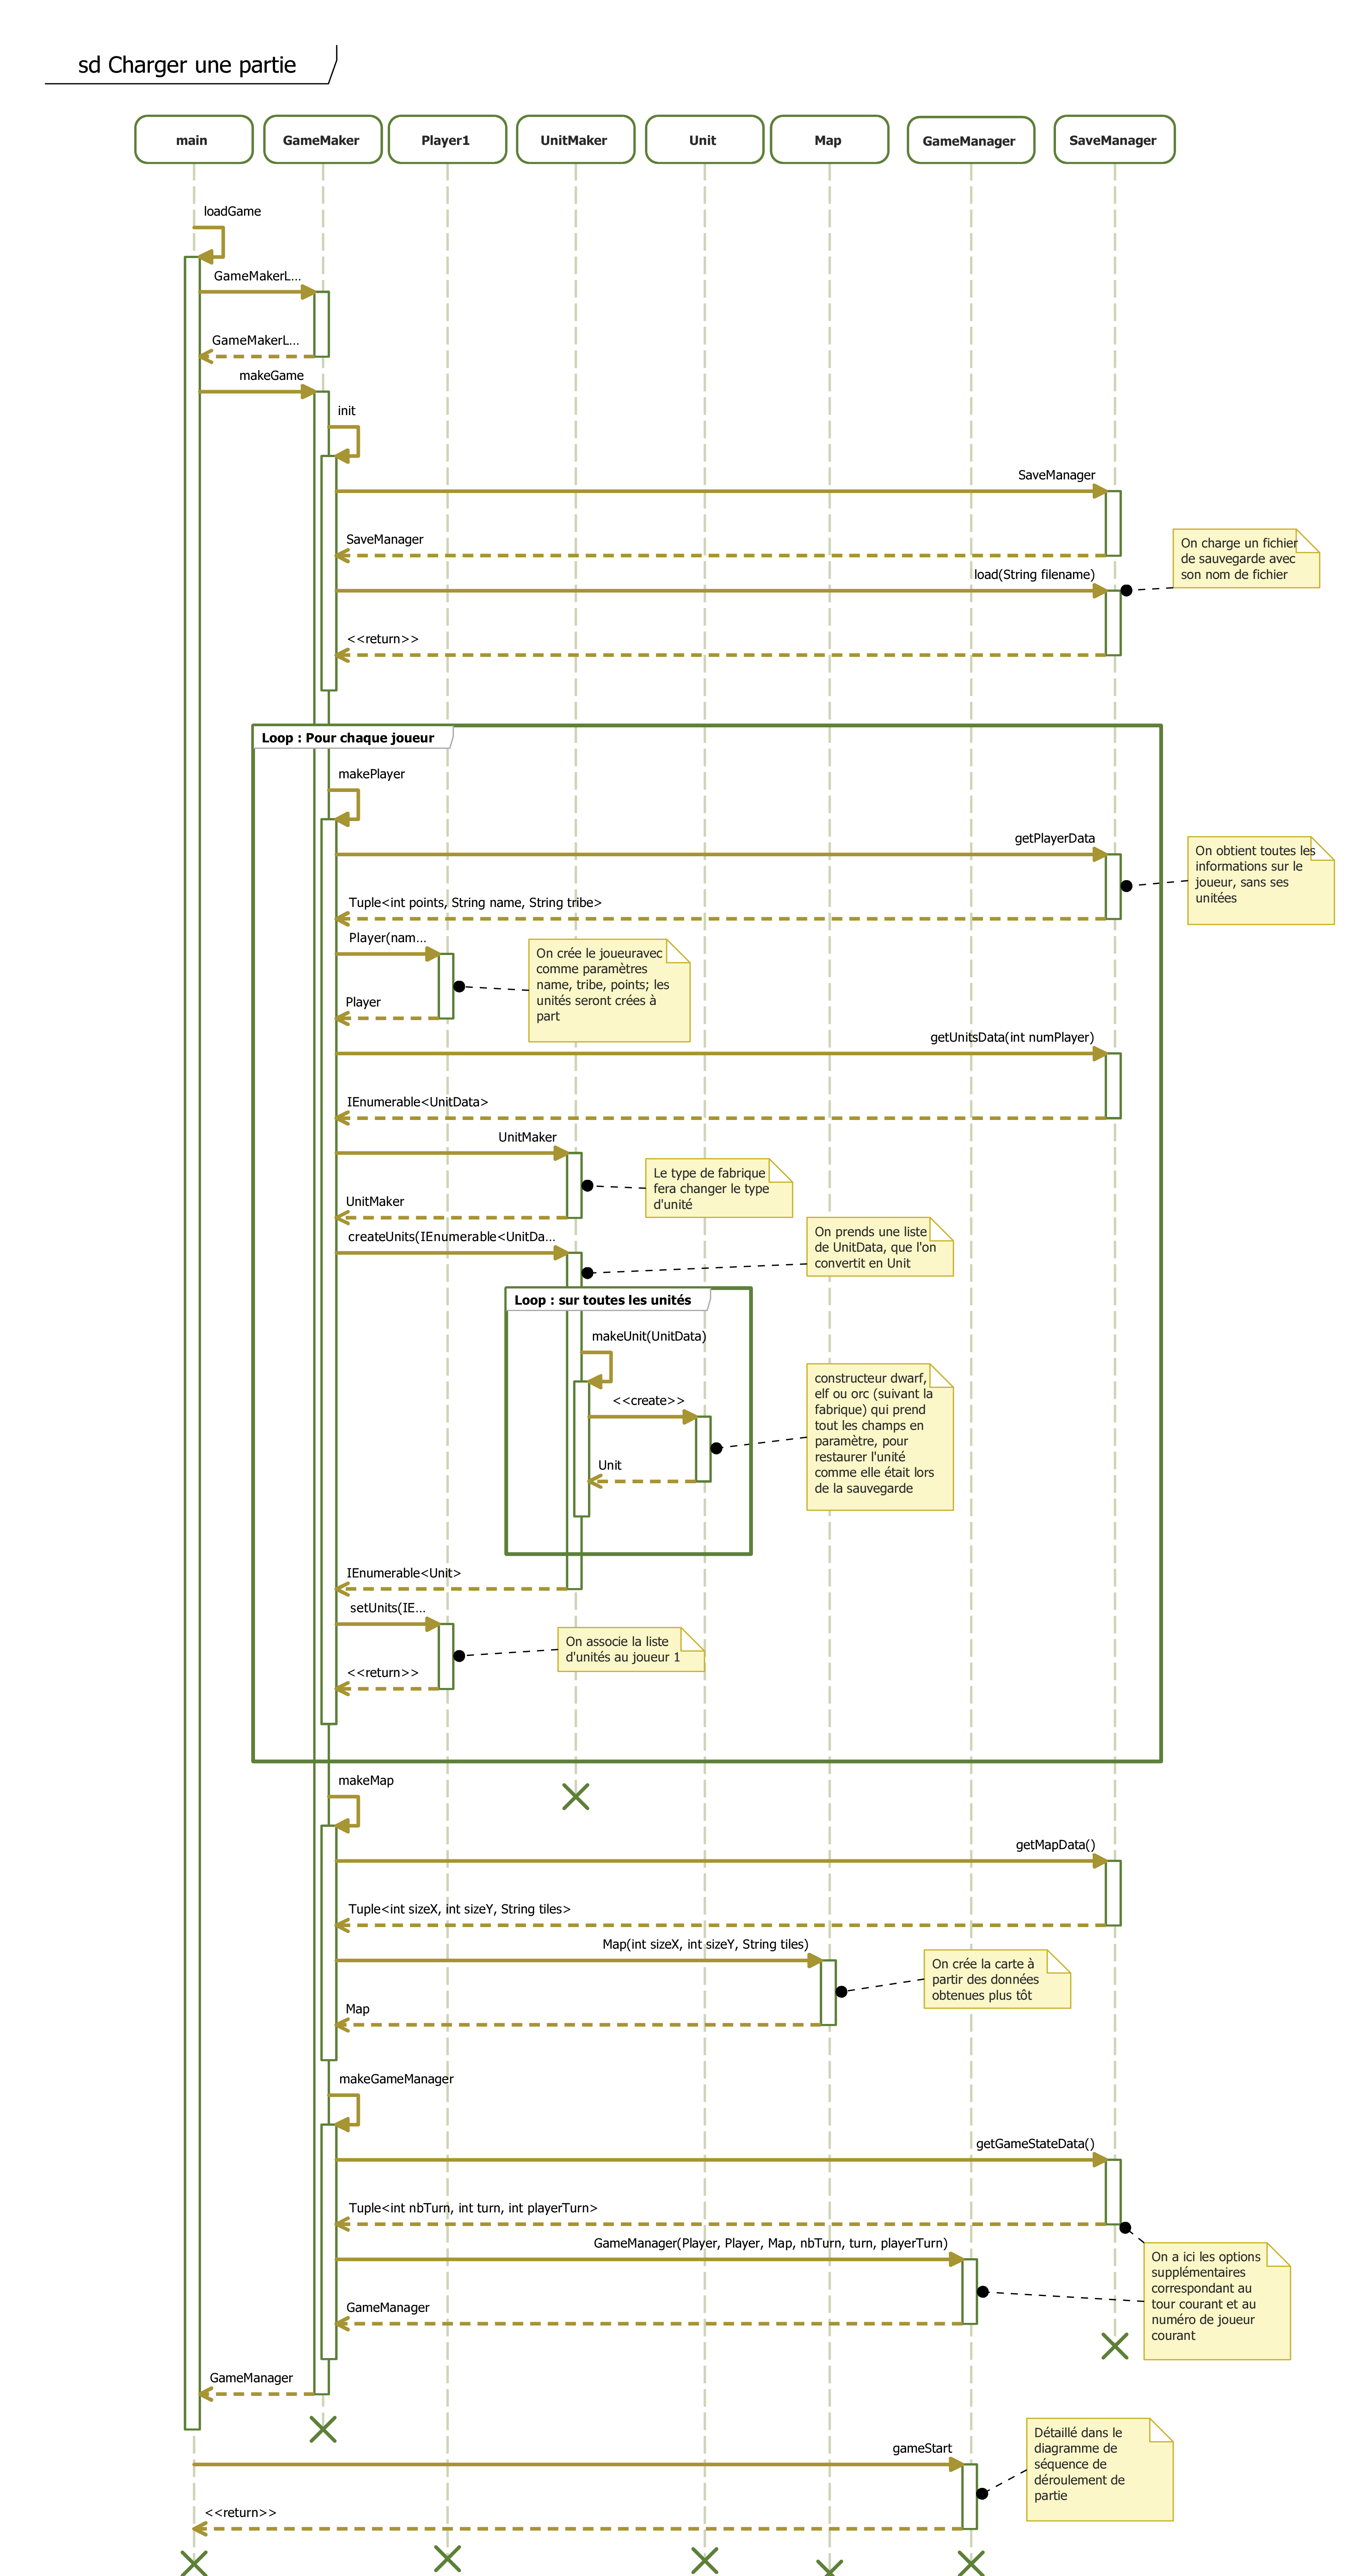
\includegraphics[width=0.8\textwidth]{res/ChargerPartie.png}
    \caption{Chargement de partie}
    \label{fig:loadGame}
\end{figure}
